\documentclass[12pt]{article}

\newcommand{\CiteMathPackage}{../../math}
\newcommand{\CiteReference}{../reference.bib}

% Packages
\usepackage{setspace,geometry,fancyvrb,rotating}
\usepackage{marginnote,datetime,enumitem}
\usepackage{titlesec,indentfirst}
\usepackage{amsmath,amsfonts,amssymb,amsthm,mathtools}
\usepackage{threeparttable,booktabs,adjustbox}
\usepackage{graphicx,epstopdf,float,soul,subfig}
\usepackage[toc,page]{appendix}
\usdate

% Page Setup
\geometry{scale=0.8}
\titleformat{\paragraph}[runin]{\itshape}{}{}{}[.]
\titlelabel{\thetitle.\;}
\setlength{\parindent}{10pt}
\setlength{\parskip}{10pt}
\usepackage{Alegreya}
\usepackage[T1]{fontenc}

%% Bibliography
\usepackage{natbib,fancybox,url,xcolor}
\definecolor{MyBlue}{rgb}{0,0.2,0.6}
\definecolor{MyRed}{rgb}{0.4,0,0.1}
\definecolor{MyGreen}{rgb}{0,0.4,0}
\definecolor{MyPink}{HTML}{E50379}
\definecolor{MyOrange}{HTML}{FF5733}
\newcommand{\highlightR}[1]{{\emph{\color{MyRed}{#1}}}} 
\newcommand{\highlightB}[1]{{\emph{\color{MyBlue}{#1}}}}
\newcommand{\highlightP}[1]{{\emph{\color{MyPink}{#1}}}}
\newcommand{\highlightO}[1]{{\emph{\color{MyOrange}{#1}}}}
\usepackage[bookmarks=true,bookmarksnumbered=true,colorlinks=true,linkcolor=MyBlue,citecolor=MyRed,filecolor=MyBlue,urlcolor=MyGreen]{hyperref}
\bibliographystyle{econ}

%% Theorem Environment
\theoremstyle{definition}
\newtheorem{assumption}{Assumption}
\newtheorem{definition}{Definition}
\newtheorem{theorem}{Theorem}
\newtheorem{proposition}{Proposition}
\newtheorem{lemma}[theorem]{Lemma}
\newtheorem{example}{Example}
\newtheorem{corollary}[theorem]{Corollary}
\usepackage{mathtools}
\usepackage{\CiteMathPackage}

\begin{document}


%-%-%-%-%-%-%-%-%-%-%-%-%-%-%-%-%-%-%-%-%-%-%-%-%-%
%-% Title
%-%-%-%-%-%-%-%-%-%-%-%-%-%-%-%-%-%-%-%-%-%-%-%-%-%

\title{\bf Where Have the Middle-Wage Workers Gone? A Study of Polarization Using Panel Data, Journal of Labor Economics, 2016}
\author{Wenzhi Wang \thanks{This note is written in my MPhil period at the University of Oxford.} } 
\date{\today}
\maketitle

\citet{cortesWhereHaveMiddleWage2016}

%??%??%??%??%??%??%??%??%??%??%??%??%??%??%??%??%??%??%??
%?? Introduction
%??%??%??%??%??%??%??%??%??%??%??%??%??%??%??%??%??%??%??

\section{Introduction}

In this paper, I investigate the implications of routine-based technical change (RBTC) within the context of a general equilibrium model with endogenous sorting of workers into occupations based on comparative advantage. The novel aspect of the paper is the focus on the individual-level predictions in terms of occupational switching patterns and wage changes. The paper's main contributions are to formalize these individual-level predictions within this type of model and to test them using data from PSID from 1976 to 2007. To the best of my knowledge, the paper is the first to directly use individual-level panel data to study the labor market experience of routine workers in the US over the past 3 decades, thus shedding light on what has happened to these workers over time. The approach taken in this paper provides evidence on (i) the micro-level dynamics underlying the aggregate patterns of employment and wage polarization, (ii) the way in which particular subsets of workers have been affected by routinization, and (iii) the changes that have occurred over time in the occupational wage premia once selection into occupations has been accounted for. 

Technology has long been considered as a potential driver of changes in the economy's employment and wage structure, but only recently has technological change been linked to occupations and their task content through theories of RBTC. Empirical studies of the effects of RBTC for the US have so far relied on repeated cross-sectional data and have studied the effects of technological change on the wage structure of the economy through changes in the occupational composition of employment. Less is known about the ways in which specific subsets of workers have been affected by RBTC. In this paper, I go a step further by using individual-level panel data in order to directly study the labor market experience of routine workers, thus providing information on their occupational mobility patterns and the wage changes they experience both in the short run and the long run. 

The empirical strategy followed in this paper also makes it possible to study the changes over time in the occupation wage premia in the US. In contrast to the focus in the earlier skill-biased technical change literature on the evolution of the skill premium, changes in occupational wage premia implied by RBTC have not received much attention. This paper fills this gap in the literature, and in the process it provides a methodological contribution by outlining a method for the unbiased and consistent estimation of changes over time in occupational wage premia after controlling for selection into occupations based on observable and unobservable individual characteristics. 

The focus on the individual-level effects of RBTC helps bridge a gap between the aggregate-level literature on polarization and the individual-level literature on occupational mobility and its associated wage changes. This individual-level literature has been expanding in recent years, focusing both on the rates of occupational mobility and on the implications of occupational transitions for individuals' human capital and wages. 

This papers contribute to this individual-level strand of literature by focusing specifically on transitions out of a rapidly declining occupational category and considering both the short-run and long-run wage effects of these transitions. Moreover, the framework presented in this paper helps interpret many of the findings from this individual-level literature within the broader context of technological change and labor market polarization. 

This paper begins by describing a model that features an occupational sorting mechanism that follows \citet{gibbonsComparativeAdvantageLearning2005}: workers select into occupations based on their comparative advantage. The model economy is composed of three distinct occupations (nonroutine manual, routine, and nonroutine cognitive) and a continuum of worker differentiated according to their skill level. Capital enters the production function as a substitute for labor working in routine tasks and as a complement for workers in nonroutine tasks. 

I derive the model's predictions for the effects of RBTC on individual workers. Routine-biased technical change is modeled as an exogenous increase in the use of physical capital (due, e.g., to a fall in the cost of computing power). The model makes the following predictions: \highlightP{RBTC induces workers at the bottom of the ability distribution within routine occupations to switch to nonroutine manual jobs, while it induces those at the top to switch to nonroutine cognitive jobs.} The model also makes predictions in terms of the changes in occupational wage premia: \highlightP{the wage premium in routine occupations is predicted to fall relative to that in the two nonroutine occupations.} For this reason, workers staying in routine jobs experience a fall in wages relative to those staying in either nonroutine manual or nonroutine cognitive jobs. At the same time, the model predicts \highlightP{that switchers must do at least as well as stayers in terms of wage growth}. These model predictions can also be derived from a more general setting with two-dimensional skills.

To test the predictions of the model for individual workers, the paper uses data from the PSID, which tracks individuals over time, making it possible to document the likelihood of transitions between different types of jobs and to analyze the wage profiles for workers with different labor market experiences. Occupations are grouped into the three categories used in the model through an aggregation of three-digit occupation codes. \footnote{All service occupations are categorized as nonroutine manual; sales and clerical occupations, craftsmen, foremen, operatives and laborers are categorized as routine; and professional and managerial occupations are categorized as nonroutine cognitive.}

The empirical strategy involves the estimation of a wage equation that is obtained directly from the model. An individual worker's potential wage in each occupation consists of an occupation-specific premium (common to all workers in the same occupation in a given year), as well as an occupation-specific return to the worker's skills. Empirically, skills are allowed to contain both observable and unobservable components. Workers select into the occupation where their potential wage is highest. The key identifying assumptions for the estimation of the wage equation are that \highlightO{(i) unobservable skills and their return are time-invariant, (ii) workers have full information about their skills, and (iii) any idiosyncratic temporary shocks to individual wages are independent of sectoral choice}. Under these assumptions, estimating a wage equation with \highlightB{occupation spell fixed effects}, i.e., interactions of individual fixed effects with occupation dummies, controls for the self-selection of workers into occupations based on unobserved ability and allows for the consistent estimation of the changes over time in the occupation wage premia. The estimated occupation spell fixed effects themselves are also informative, as they can be used to rank workers according to ability within occupation-year cells. The empirical specification can allow for variation over time in observable skills or in the return to education, as well as for cots to occupational mobility due to the loss of occupation or task-specific human capital. 

The results indicate that there is strong evidence of selection on ability for workers switching out of routine jobs: low-ability routine workers are more likely to switch to nonroutine manual jobs, while high-ability routine workers are more likely to switch to nonroutine cognitive jobs. This is fully consistent with the predictions of the model. 

In terms of the wage growth, I find that workers staying in routine jobs perform significantly worse than workers staying in any other type of occupation. The wage premium for routine occupations is estimated to have fallen by 17\% from 1976 to the mid-2000s relative to the wage premium for nonroutine manual occupations. Meanwhile, over the same time period, the wage premium for nonroutine cognitive occupations is estimated to have risen by 25\% relative to the wage premium for nonroutine manual occupations. The fall in the wage premium in routine occupations is not explained by changes in the return to education or by lower returns to occupational tenure in routine jobs. 

There are also significant differences in wage growth between routine workers who stay in routine jobs and those who switch to other occupations: Workers switching to nonroutine manual jobs have significantly lower wage growth than stayers over short-run horizons (around 14\% lower over a 2-year period), but they subsequently recover from these losses and have significantly faster wage growth than stayers in the long run (5\%-12\% higher over a 10-year period). Meanwhile, those who switch to nonroutine cognitive occupations have significantly higher wage growth than stayers over all time horizons (6\%-12\% higher over a 2-year period; 14\%-16\% higher over a 10-year period). The results are robust to accounting for subsequent occupational switches and attrition.

%??%??%??%??%??%??%??%??%??%??%??%??%??%??%??%??%??%??%??
%?? Model
%??%??%??%??%??%??%??%??%??%??%??%??%??%??%??%??%??%??%??

\section{The Model}

There is a single representative household composed of a continuum of workers, who differ in terms of their skill levels. There is perfect information, and workers sort endogenously into one of three occupations. The three occupations are labelled as nonroutine manual ($M$), routine ($R$), and nonroutine cognitive ($C$).

Occupation sorting is driven by comparative advantage. Specifically, workers of higher skill levels are assumed to be more productive at all tasks, but particularly so at more complex tasks (where nonroutine cognitive tasks are assumed to be the most complex and nonroutine manual the least complex). Letting $z$ denote the individual's skill level and $\phi_j\of{z}$ the productivity (in terms of supplied efficiency units) of a worker of skill $z$ performing task $j \in \bc{M, R, C}$, this assumption is formalized as 
\begin{equation}
    \notag
    0 < \frac{d \log\of{\phi_M\of{z}}}{d z} < \frac{d \log\of{\phi_R\of{z}}}{d z} < \frac{d \log\of{\phi_C\of{z}}}{d z}.
\end{equation}

Potential wages for each worker in each occupation are the product of the competitively determined wage per efficiency unit in that occupation, denoted $\l_j$, and the number of efficiency units supplied by the worker. That is, $w_j\of{z} = \l_j \phi_j\of{z}$, where $w_j\of{z}$ is the potential wage in occupation $j \in \bc{M, R, C}$ for an individual of skill level $z$.

In equilibrium, there will be two endogenously determined skill thresholds, $z_0$ and $z_1$, such that the least skilled workers will find it optimal to select into the nonroutine manual occupation, the middle-skill workers into the routine occupation, and the most skilled workers into the nonroutine cognitive occupation.

The equilibrium relationship between skills, occupational choices, and wages is depicted in part a of figure \ref{fig1}, under the assumption that productivity is log-linear in skills. The three lines depict potential wages in each of the three occupations. The slope of the potential wage curve is lowest in the nonroutine manual occupation and highest in the nonroutine cognitive one, reflecting the assumption that productivity increases fastest with skills in the nonroutine cognitive occupation.

The intercepts of the three curves correspond to the wage per efficiency unit in each of the three occupations. Intuitively, if the wages per efficiency unit were the same for all three tasks, i.e., $\l_C = \l_R = \l_M$, all workers would want to sort into the nonroutine cognitive occupation. However, it can be shown that, in equilibrium, demand for all tasks is positive; therefore, it must be the case that, in equilibrium, $\l_C$ is relatively low, while $\l_M$ must be relatively high. The low $\l_C$ makes it optimal only for the most skilled workers to select into the nonroutine cognitive occupation (where they are much more productive), while the high $\l_M$ attracts the least skilled workers to the nonroutine manual occupation (as their extra productivity in the other tasks is relatively small).

\begin{figure}[H]
    \noindent
    \caption{Equilibrium relationship between skills, occupational choice and wages, and effects of routine-biased technical change}
    \centerline{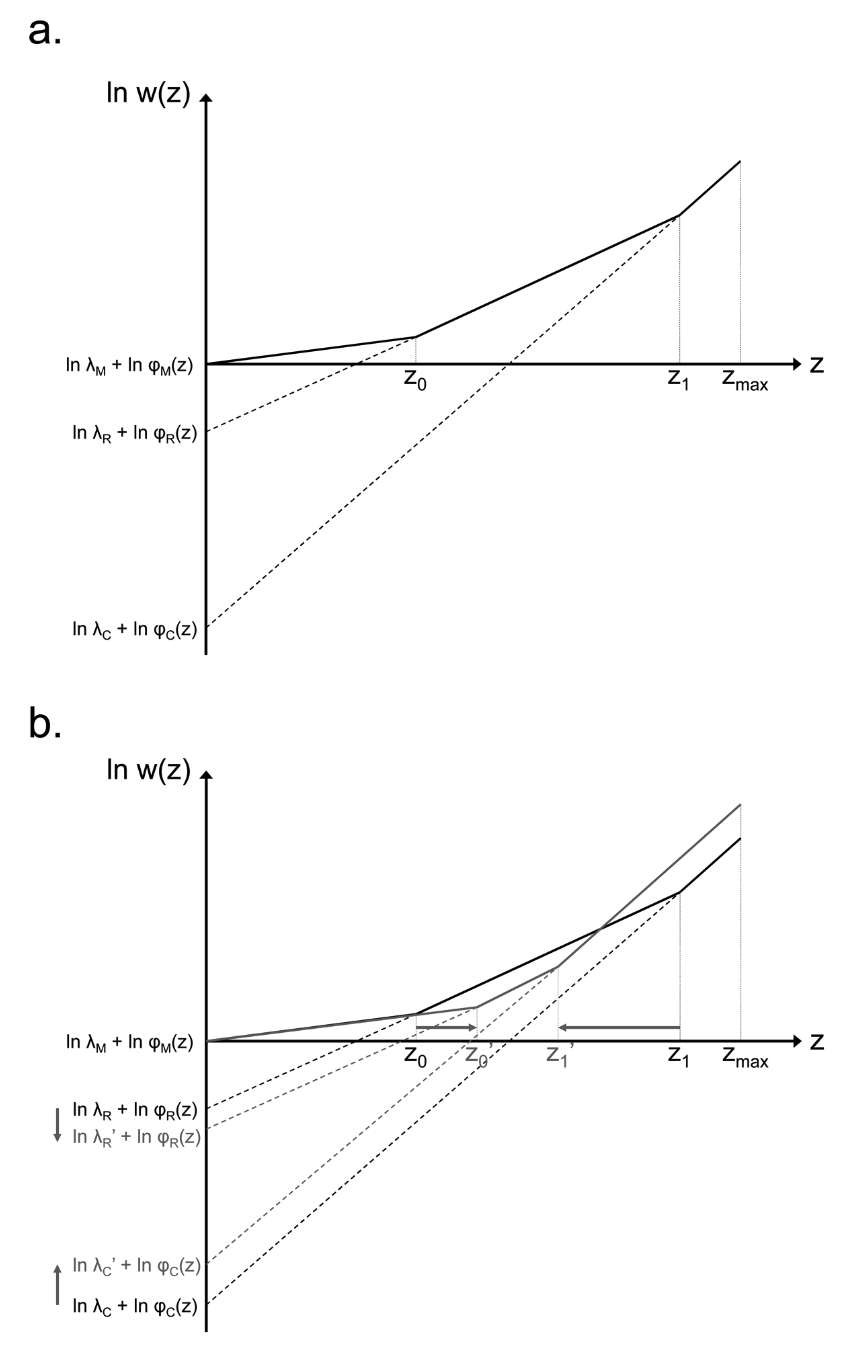
\includegraphics[scale=0.6]{cortes2016_fig1.png}}
    \label{fig1}
\end{figure}

On the production side of the model, there are two consumption goods that use the different tasks as inputs. The representative household has Cobb-Douglas preferences over the two goods. The first good is a ``service good,'' which is produced using only labor performing nonroutine manual tasks. The second is a ``manufactured good,'' which has a production function that features complementarities between routine and nonroutine cognitive task services. Routine task services are supplied by labor and by physical capital, while nonroutine cognitive tasks are performed only by labor. Thus, capital enters the production function as a complement for workers performing nonroutine cognitive tasks and as a substitute for workers performing routine tasks. Capital is exogenous and assumed to be available at no cost.

Technical change is modelled as an exogenous increase in the capital stock. This shock reduces the relative demand for labor performing routine tasks and is therefore referred to as ``routine-biased'' technical change. The effect of RBTC on the equilibrium of the model are illustrated in part b of figure \ref{fig1}.

Consider, first, the effect of an increase in the capital stock on the wages per efficiency unit in each occupation. \highlightP{The immediate effect of the shock is to increase the relative demand for nonroutine cognitive tasks within the manufacturing sector due to the complementarities between routine and nonroutine cognitive task services.} This increases the wage per efficiency unit in those occupations relative to routine ones. \highlightP{Meanwhile, there is an increase in household income, which increases the demand for the the service good. This pushes up the wage per efficiency unit in the nonroutine manual occupation relative to the wages per efficiency unit in the other occupations.}

The figure also shows the implications in terms of the occupational composition of employment. The increased demand for nonroutine workers causes an expansion of both types of nonroutine employment and a contraction of routine employment. This is the essence of job polarization.

We can also determine who switches out of routine jobs. As the skill cutoff between routine and nonroutine cognitive tasks falls, the highest-ability routine workers will be the ones who find it optimal to switch to nonroutine cognitive jobs (due to comparative advantage). Meanwhile, the increase in the skill cutoff between nonroutine manual and routine tasks implies that it is the lowest-ability routine workers who find it optimal to switch to nonroutine manual tasks.

Finally, consider the total wage changes for workers of different ability levels. Workers who do not find it optimal to switch occupations simply experience a wage change equal to the change in the wages per efficiency unit in their optimal occupation. Workers switching out of routine jobs must do at least as well as those who stay, as they could have chosen to stay in the routine occupation but find it optimal not to do so.

To summarize, the general equilibrium effects of RBTC are these: 
\begin{enumerate}[topsep=0pt, leftmargin=20pt, itemsep=0pt, label=(\arabic*)]
    \setlength{\parskip}{10pt} 
    \item Workers at the bottom of the ability distribution within routine occupations switch to nonroutine manual jobs, workers at the top of the ability distribution within routine occupations switch to nonroutine cognitive jobs, and no switching is induced for nonroutine workers (either manual or cognitive).
    \item Workers staying in routine jobs experience a fall in real wages relative to those staying in other jobs, and workers staying in nonroutine cognitive jobs experience an increase in real wages relative to those staying in other jobs.
    \item Workers who switch from routine to nonroutine jobs (either manual or cognitive) experience an increase in real wages relative to those who stay in the routine occupation.
\end{enumerate}

\highlightR{WWZ Notes: The implications are derived by settings which initially imply that routine-biased technical change increases relative wage of nonroutine cognitive occupations while decreases relative wage of routine occupations.}

The theoretical model sketched above assumes that workers' skills are one-dimensional. The simple intuition obtained from this model can also be derived (in expectations) from a richer model where workers have two-dimensional skill endowments (cognitive and manual). Heterogeneities across age groups could be introduced by allowing for changes over the life cycle in worker skills or in worker productivities in the different occupations. Conditional on the wages per efficiency unit in each occupation, occupational choice in this model depends only on skills. In this sense, the model differs from models where occupational choice is driven also by uncertainty or idiosyncratic match qualities. 

\highlightO{Another abstraction made by the model is that it assumes that there is no cost to switching occupations.} Intuitively, if we allowed for a positive cost for switches into nonroutine cognitive occupations (e.g., because of educational requirements,) then the RBTC shock would induce fewer workers to switch to this occupation, and those who do switch would be a more positively selected subset. Depending on how this cost is modeled, it would also have implications for the equilibrium conditions of the model. 

\section{Empirical Implementation}

From the model, the potential wage for an individual of skill level $z_i$ in occupation $j$ consists of an occupation wage premium $\l_j$, which is common to everyone in the occupation, and on the individual's occupation-specific productivity $\f_j\of{z_i}$. Assume that productivity is log-linear in skills, that is, 
\begin{equation}
    \label{1}
    \ln \f_j\of{z_i} = z_i \a_j,
\end{equation}
where $\a_j$ may be interpreted as an occupation-specific return to skills. Following the assumptions on comparative advantage from the model, assume that these occupation-specific returns are highest in the nonroutine cognitive occupation and lowest in the nonroutine manual one. That is, 
\begin{equation}
    \notag 
    \a_M < \a_R < \a_C.
\end{equation}
This assumption reflects the fact that skill premia vary across occupations, leading to workers of different abilities selfselecting into different occupations, as described in the model.

Using the assumed functional form for productivity and allowing for variation over time in the occupation wage premium (e.g., because of RBTC), we have the following equation for the potential wage in occupation $j$ for individual $i$ of skill level $z_i$:
\begin{equation}
    \label{2}
    \ln w_{ijt} = \t_{jt} + z_i \a_j,
\end{equation}
where $i$ denotes the individual, $j$ denotes the occupation, $t$ denotes the time period, and $\t_{jt} \equiv \ln \l_{jt}$ is the occupation wage premium in occupation $j$ at time $t$. Note that I am assuming that individual skills are time-invariant. This assumption will be relaxed later on to allow for certain types of timevarying skills.

The wage observed by the econmetrician for individual $i$ in period $t$ will depend on the occupation chosen by the individual and will be given by 
\begin{equation}
    \label{3}
    \ln w_{it} = \sum_{j} D_{ijt} \t_{jt} + \sum_{j} D_{ijt} z_i \a_j + \mu_{it},
\end{equation}
where $D_{ijt}$ is an occupation selection indicator that equals one if person $i$ selects into occupation $j \in \bc{M, R, C}$ at time $t$ and zero otherwise, and $\mu_{it}$ reflects classical measurement error, which is assumed to be independent of sector affiliation and therefore orthogonal to $D_{ijt}$. The term $\mu_{it}$ may also be interpreted as a temporary idiosyncratic shock that affects the wages of individual $i$ in period $t$ regardless of his occupational choice.

Without any restrictions to mobility, a worker will select into the occupation where he receives the highest wage. Given a fixed $\t_{jt}$, there will exist critical values of $z_i$ that determine the efficient assignment of workers to occupations. Because $z_i$ and $\a_j$ are not varying over time, and because $\mu_{it}$ is not occupation-specific, occupational mobility will be driven exclusively by changes over time in $\t_{jt}$. 

In practice, occupational mobility is not frictionless. One can think of a worker's occupational choice as being driven by $z_i$ and $\t_{jt}$, as well as a noise component that is uncorrelated with wages. This noise component may be interpreted as a search friction that does not affect a worker's potential wage in the different occupations but that restricts the worker from immediately selecting into his desired occupations each period. Put differently, the identifying assumption is that, conditional on the occupation fixed effects and on individual workers' skills, selection into occupations is random, i.e., driven by a search friction that is orthogonal to skills or to any other wage determinants. Thus, we assume that in equation (\ref{3}),
\begin{equation}
    \notag 
    \E\bs{\mu_{it} \mid D_{ijt}, z_i, \t_{jt}} = 0.
\end{equation}
This assumption rules out dynamic effects such as workers learning about their ability over time. The assumption also rules out that different types of switches may have different costs (e.g., because of differences in task distances across occupations), or that switching may be more costly for workers with higher levels of occupational tenure (because of the importance of occupation-specific human capital).

Given that I am not interested in identifying $\a_j$ (the occupation-specific return to skills), I rewrite equation (\ref{3}) as 
\begin{equation}
    \label{4}
    \ln w_{it} = \sum_{j} D_{ijt} \t_{jt} + \sum_{j} D_{ijt} \g_{ij} + \mu_{it},
\end{equation}
where $\g_{ij} \equiv z_i \a_j$. The term $\g_{ij}$ is composed of an individual's time-invariant skills and the occupation-specific returns to those skills; $\g_{ij}$ varies for an individual across occupation spells, but it stays constant whenever the individual stays in the same occupation. Equation (\ref{4}) can be consistently estimated using fixed effects at the occupation spell level for each individual, i.e., using a fixed effect for each individual in each occupation that they are observed in. The fixed effects demeans wages for each individual within occupation spells, thus capturing the time-invariant component within the spell, which is precisely the unobserved effect $\g_{ij}$. Recall that $z_i$ (through the fixed effect $\g_{ij}$) and $\t_{jt}$ are controlled for, selection into occupations is random (depends only on the search friction). Therefore, the regressors in equation (\ref{4}) are orthogonal to the mean-zero error term $\mu_{it}$ and the coefficients are consistently estimated. 

In the empirical estimation, $\t_{jt}$ is captured with interactions of occupation and year dummies. The omitted category in all years is the nonroutine manual occupation, and all wages are relative to this normalization. To capture changes over time that affect all occupations (including nonroutine manual) and to ensure that the normalization of $\t_{M, t}$ to zero in all years is appropriate, the estimation includes a set of aggregate year effects that are assumed to all workers, regardless of their occupation or skill level. The estimates of $\t_{R,t}$ and $\t_{C,t}$ will reflect changes in the occupation wage premium over time, due to RBTC or other shocks, relative to the base occupation. \highlightP{Because of the inclusion of the occupation spell fixed effects, the occupation-time fixed effects are identified only from variation over time within occupation spells.} Therefore, it is necessary to normalize $\t_{R, t}$ and $\t_{C,t}$ to zero for a base year. This identification argument implies that $\wh{\t}_{R, t}$ and $\wh{\t}_{C, t}$ should be interpreted as estimating a double difference: \highlightP{rather than identifying the level of the occupation wage premia, they identify their changes over time relative to the base year and relative to the analogous change experienced by the base occupation (nonroutine manual).} As the purpose of this paper is to analyze changes over time in occupational wage premia, rather than their level, these are in fact the parameters of interest.

The estimation procedure also makes it possible to generate estimated occupation spell fixed effects $\wh{\g}_{ij}$. They will be an estimator of the return to time-invariant skills for individual $i$ conditional on selecting into occupation $j$. Because $\g_{ij}$ is monotonically increasing in skill within the occupation (the coefficient on skills is common for all workers who select into the occupation), \highlightP{the ranking of workers according to this measure corresponds to their ranking according to their underlying ability}. In order to test the model's implications regarding switching patterns, I am only interested in a worker's relative ability within an occupation in a given year, so having an estimator with which I can rank workers conditional on having selected into an occupation is sufficient for my purposes.

When estimating equation (\ref{4}) in the data, I add an extra set of controls for marital status, unionization status, region of residence, and a dummy for whether the individual lives in a metropolitan area (SMSA). It is assumed that these variables are orthogonal to the measurement error mit and that their return is not occupation-specific or skill-specific. Their inclusion will therefore not affect the consistency of the estimated coefficients.

To summarize, the equation being estimated is
\begin{equation}
    \label{5}
    \ln w_{it} = \sum_{j} D_{ijt} \t_{jt} + \sum_{j} D_{ijt} \g_{ij} + \bds{Z}_{ij}^{\prime} \bds{\zeta} + \mu_{it},
\end{equation}
where $\t_{jt}$ are occupation-time fixed effects, $\g_{ij}$ are occupation spell fixed effects for each individual, and $\bds{Z}_{ij}$ includes year fixed effects and controls for marital status, unionization status, region of residence, and SMSA. In all the estimations, standard errors are clustered at the individual level.





\bibliography{\CiteReference}


\end{document}
